%! TEX program = lualatex
\documentclass[10pt, a4paper]{beamer} %handout fuer eine gedruckte version der slides
\usetheme{metropolis}

\usepackage{url}
\usepackage{polyglossia}
\setmainlanguage{english}

\usepackage{listings,xcolor}
\usepackage{graphicx}
\usepackage{nameref}
\usepackage{mathtools}

\usepackage{booktabs}

\makeatletter
\newcommand*{\currentname}{\@currentlabelname}
\makeatother

\usepackage{fontspec}
% \setmainfont{UbuntuMono}
\newfontfamily\Bera{PragmataPro Mono Liga}[Scale=0.85]

\definecolor{mDarkTeal}{HTML}{23373b}
\definecolor{mLightBrown}{HTML}{EB811B}
\definecolor{mDarkBlue}{HTML}{0F3470}
\definecolor{mDarkGrey}{HTML}{999999}
\definecolor{mLighterGrey}{HTML}{CCCCCC}
\definecolor{mLightGrey}{rgb}{0.95,0.95,0.95}
\definecolor{mLightBlue}{HTML}{212751}

\newcommand{\lb}[1]{{\color{mLightBrown}#1}}

\newcommand{\bblock}[3]{
    \begin{block}{#1}
    #2
  \end{block}
}

\setbeamercolor{block title}{fg=mDarkTeal}

\lstset{language=Python,
  backgroundcolor=\color{mLightGrey},
  frame=single,
  rulecolor=\color{mLightGrey}, % make frame "invisible"
  basicstyle=\Bera\footnotesize,
  keywordstyle=\bfseries\color{mDarkBlue},
  commentstyle=\color{mDarkGrey}\itshape,
  captionpos=t,
  emphstyle=\ttb\color{mDarkBlue},  % Custom highlighting style
  stringstyle=\color{mLightBrown},
  tabsize=2,
  numberbychapter=false,
  showstringspaces=false,
  breaklines=true,
  morekeywords={__init__, and, assert, break, class, continue, def, del, elif, else, except, exec, finally, for, from, global, if, import, in, is, lambda, not, or, pass, print, raise, return, try, while, yield}
}
%
\makeatletter
\setbeamertemplate{footline}{%
\leavevmode
\vbox{\begin{beamercolorbox}[dp=1.25ex,ht=2.75ex]{fg=black}%
  \hspace*{1em}\insertsectionhead%
  \ifx\insertsubsectionhead\@empty\relax\else\hspace*{\fill}\insertsubsectionhead\hspace*{2ex}\fi
  \end{beamercolorbox}%
  }%
}
\makeatother

\setbeamertemplate{section in toc}{%
  {\color{mDarkTeal}\rule[0.3ex]{3pt}{3pt}}~\inserttocsection\par}
\setbeamertemplate{subsection in toc}{%
  \hspace{1.2em}{\color{mLightBrown}\rule[0.3ex]{3pt}{3pt}}~\inserttocsubsection\par}


% \usecolortheme{spruce}
\AtBeginSubsection[]
{
  {
%   \setbeamercolor{background canvas}{bg=mLighterGrey}
  \begin{frame}
    \centering\bfseries\Large\currentname
  \end{frame}
  }
}

\title % (optional, only for long titles)
{Python Basics}
\author % (optional, for multiple authors)
{Philipp Gloor\inst{1}}
\institute
{
  \inst{1}%
  University of Zurich
}
\date{}
\subject{Python}
\titlegraphic{
\includegraphics[width=0.3\textwidth]{pics/uzh_logo_e_pos}}
\begin{document}
\begin{frame}
  \titlepage
\end{frame}

\begin{frame}{Table of Contents}
  \tableofcontents
\end{frame}
\section{General Introduction}
\begin{frame}
  \frametitle{About me}

  \begin{block}{Education}
    \begin{itemize}
      \item 2012 -- Bachelor of Science UZH in Physics
      \item 2016 -- Master of Science UZH in Computational Science
    \end{itemize}
  \end{block}

  \begin{block}{Work}
    \begin{itemize}
      \item 2014 -- 2016: Software engineer CERN (remote)
      \item 2016 -- 2021: PDF Tools AG
      \item 2021 -- now: Zurich Instruments
    \end{itemize}
  \end{block}

  \begin{block}{Programming experience}
    \begin{itemize}
      \item[] C++, C\#, Java, TypeScript, JavaScript, Python
    \end{itemize}
  \end{block}

  \begin{block}{Email}
    \begin{itemize}
      \item[] philipp.gloor@protonmail.com
    \end{itemize}

  \end{block}

  % In this slide, some important text will be
  % \alert{highlighted} beause it's important.
  % Please, don't abuse it.

  % \begin{block}{Remark}
  % Sample text
  % \end{block}

  % \begin{alertblock}{Important theorem}
  % Sample text in red box
  % \end{alertblock}

  % \begin{examples}
  % Sample text in green box. "Examples" is fixed as block title.
  % \end{examples}
\end{frame}
% \begin{frame}[c]\frametitle{Round of introduction}
%   \begin{itemize}
%     \item Name
%     \item Occupation
%     \item Programming experience? What language?
%     \item Expectations
%   \end{itemize}
% \end{frame}

\begin{frame}[c]\frametitle{Learning targets}

  After this course...
  \begin{itemize}
    \item ... you will have an idea what programming is
    \item ... you will know how to write a basic computer program
    \item ... you are able to write a Python program based on a written out
          problem statement
    \item ... you know where you can find more information to improve your
          programming skills
  \end{itemize}

  But you only have started to scratch the surface.
\end{frame}


\section{Introduction to Programming} % (fold)
\label{sec:introduction_to_programming}

\begin{frame}[c]\frametitle{What is a Computer Program}
  \begin{block}{Modular System}
    \begin{itemize}
      \item \textbf{Input}: Data input from keyboard, files, internet, etc...
      \item \textbf{Output}: Processed data is displayed or saved to a file
      \item \textbf{Algorithms}: The computers cooking recipies
      \item \textbf{Libraries}: Using existing implementations (can do anything of the above)
    \end{itemize}

  \end{block}
\end{frame}

\begin{frame}[c]\frametitle{Why Python?}
  \begin{columns}
    \begin{column}{0.5\textwidth}
      \begin{itemize}
        \item High-level programming language
        \item "Simple" syntax
        \item Cross-platform - A script written on a Windows computer also runs on Linux \& Mac
        \item Interpreted => Easy to run
              % \item Object-oriented
        \item Many libraries available
      \end{itemize}
    \end{column}
    \begin{column}{0.5\textwidth}  %%<--- here
      \begin{figure}
        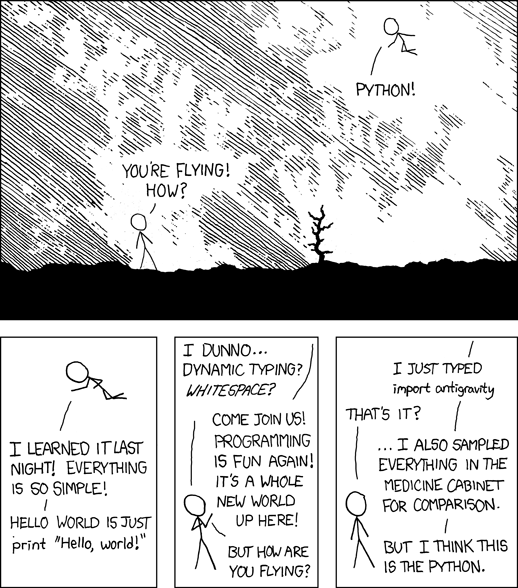
\includegraphics[width=0.9\linewidth]{pics/python.png}
      \end{figure}
      \tiny Source: https://xkcd.com/353/
    \end{column}
  \end{columns}

\end{frame}

\begin{frame}[fragile,c,allowframebreaks]\frametitle{Examples: Hello World}
  High level languages but not trivial to learn:
  \begin{block}{Java}
    {
      % \lstset
      \begin{lstlisting}[language=Java]
public class HelloWorld {
  public static void main(String args[]) {
    System.out.println("Hello World");
  }
}
  \end{lstlisting}
    }
  \end{block}

  \begin{block}{C++}
    {
      % \lstset
      \begin{lstlisting}[language=C++, morekeywords=include]
#include <iostream>
int main() {
  std::cout << "Hello World\n";
  return 0;
}
  \end{lstlisting}
    }
  \end{block}
  \framebreak
  Or even worse:
  \begin{block}{Machine Language}

    Example of a low level language
    \begin{lstlisting}{language=assembly}
.LC0:
  .string "Hello world!"
main:
  push rbp
  mov rbp, rsp
  mov edi, OFFSET FLAT:.LC0
  mov eax, 0
  call printf
  mov eax, 0
  pop rbp
  ret
\end{lstlisting}

  \end{block}

  \begin{block}{Python}
    \begin{lstlisting}
print("Hello World")
    \end{lstlisting}
  \end{block}

\end{frame}

\begin{frame}[fragile,c]\frametitle{How to Run Python Code}

  \begin{block}{Options to run Python code:}
    \begin{itemize}
      \item Directly in the Python prompt (REPL - Read, Eval, Print, Loop)
      \item Write the code into a file and run python with the file
      \item Use IDE to run Python code
    \end{itemize}
  \end{block}

\end{frame}

\begin{frame}[c]\frametitle{Development Environment}

  \begin{itemize}
    \item Integrated Development Environment (IDE)
    \item Collection of tools that are commonly used for software development (they make our life easier!)
    \item Popular IDEs
          \begin{itemize}
            \item Visual Studio Code - \url{https://code.visualstudio.com}
            \item JetBrains PyCharm - Community Edition available for free \url{http://jetbrains.com/pycharm/download}
            \item Eclipse with pydev - \url{http://pydev.org}
          \end{itemize}
    \item It takes time to get proficient using an IDE
  \end{itemize}
\end{frame}

% section introduction_to_programming (end)

\section{Fundamental Concepts} % (fold)
\label{sec:fundamental_concepts}

\subsection{Types, Variables, Expressions, Operators, Comments} % (fold)
\label{sub:Types_variables_expressions_operators_comments}

\begin{frame}[c]\frametitle{Data Types, Variables, Expressions, Operators, Comments}
  \begin{block}{Types}
    \begin{itemize}
      \item Numbers (Integers, Floats)
            \begin{itemize}
              \item 2
              \item 1000000
              \item -2
              \item 3.2
              \item 1.3333333
            \end{itemize}
    \end{itemize}
  \end{block}

\end{frame}

\begin{frame}[c, allowframebreaks]\frametitle{Data Types}
  \begin{block}{Strings}
    \begin{itemize}
      \item Strings (Text)
            \begin{itemize}
              \item {\color{blue}'Hello World'}
              \item {\color{red}"Hello World"}
            \end{itemize}
      \item {\color{blue} 'Single quotes'} or {\color{red} "double quotes"} can be used to declare them
            \begin{itemize}
              \item 'Hello World'
              \item "Hello World"
              \item "5"
            \end{itemize}
    \end{itemize}
  \end{block}
  \begin{block}{Boolean}
    Binary data type
    \begin{itemize}
      \item True
      \item False
    \end{itemize}
  \end{block}
  \begin{block}{None Type}
    \begin{itemize}
      \item \texttt{None} is a special type (in other languages also sometimes called \texttt{null} or \texttt{nullptr}).
    Sometimes it is necessary to indicate that something \textit{is not there} and this can be indicated by using \texttt{None}.
    \end{itemize}
  \end{block}


\end{frame}

\begin{frame}[c,fragile,allowframebreaks]\frametitle{Variables}

  Variables are used to store information to be referenced and manipulated in a computer program.
  They also provide a way of labeling data with a descriptive name, so our programs can be understood more clearly by the reader and ourselves.
  It is helpful to think of variables as containers that hold information.
  Their sole purpose is to label and store data in memory.
  This data can then be used throughout your program.

  \begin{itemize}
    \item Variables hold values
    \item Similar to mathematics
          \begin{itemize}
            \item x = 2
            \item y = x + 2
          \end{itemize}
    \item Values assigned using the \texttt{=} operator
  \end{itemize}
  \begin{examples}
    Use meaningful names
    \begin{itemize}
      \item Declaration
            \begin{lstlisting}
salutation = "Hello"
name = "Monty Python"
pi = 3.14159
    \end{lstlisting}
      \item Usage
            \begin{lstlisting}
print(name)
    \end{lstlisting}
    \end{itemize}

  \end{examples}
  \framebreak
  \begin{block}{Variables and values can be combined}
    \begin{lstlisting}
a = 3
b = 8.3
c = a + b
print(c)

salutation = "Hello"
name = "Monty Python"
print(salutation + " " + name) # Keep this printing syntax in mind
    \end{lstlisting}
  \end{block}
  \framebreak
  \begin{block}{Keywords - reserved words}

    You cannot name a variable with these names as they are protected by the language.

    \begin{lstlisting}
and, assert, break, class, continue, def, del, elif, else, except, exec,
finally, for, from, global, if, import, in, is, lambda, not, or, pass,
print, raise, return, try, while, yield
\end{lstlisting}

  \end{block}
\end{frame}

\begin{frame}[t, fragile]\frametitle{Operators}
  \begin{block}{Order of precedence (kind of like PEMDAS)}
    \begin{itemize}
      \item ()
      \item **
      \item unary + -
      \item *  /  \% //
      \item binary + -
      \item \texttt{<}, \texttt{>}, \texttt{<=}, \texttt{>=}, \texttt{!=}, \texttt{==}
      \item \textbf{\texttt{\color{mDarkBlue}not}}
      \item \textbf{\texttt{\color{mDarkBlue}and}}
      \item \textbf{\texttt{\color{mDarkBlue}or}}
    \end{itemize}
  \end{block}

\end{frame}

\begin{frame}[c, fragile]\frametitle{Comments}
  \begin{itemize}
    \item Comments have no impact on the program
    \item Should explain the code
    \item A comment starts with a \# character
  \end{itemize}

  \begin{examples}
    \begin{lstlisting}
# Declaring the name
name = "Philipp"
print(name) # Prints Philipp
  \end{lstlisting}
  \end{examples}



\end{frame}

% subsection values_variables_expressions_operators_comments (end)
% \subsection*{Pretty Print - How to Print to Console in Python}


\begin{frame}[c, fragile]\frametitle{How to Print to Console in Python}
  Printing is useful to provide feedback to the user or sometimes to debug your program. Printing different data types
  in the same print statement can be cumbersome.
  \begin{itemize}
    \item \texttt{print()} is the function to print something to console in python
  \end{itemize}

  \begin{lstlisting}
print('This prints just a string')
answer = 42
print(answer)  # Just print a number
print('Combining a string and a number: ' + answer) # -> TypeError
print(f'Much cleaner way to print string and a number: {answer}')
\end{lstlisting}


\end{frame}
% subsection(pret)

\subsection{Functions in Python} % (fold)
\label{sub:functions}
\begin{frame}[c, fragile,allowframebreaks]
  \frametitle{Functions}
  Function are self contained modules of code that accomplish a specific task. They usually "accept" input data and "return" a result.
  \begin{itemize}
    \begin{lstlisting}
name = "Some name"
print(name) # Some name is used inside the print function -> the print function accepts the input and prints it to the console
    \end{lstlisting}
    \item Functions can (and often do) also return a result (but the print function does not)
          \begin{itemize}
            \item \lstinline!return! statement
            \item If a function has no explicit return statement it implicitly returns \lstinline!None!
          \end{itemize}
  \end{itemize}

  \begin{examples}
    \begin{lstlisting}
text = "Python programming language"
print(text) # Prints: Python programming language
text_length = len(text) # This function returns the length of the text
print(text_length) # Prints length of the string
  \end{lstlisting}
  \end{examples}
\end{frame}

\begin{frame}[c, fragile,allowframebreaks]
  \frametitle{Type Conversions}

  Assume you want to program a calculator.
  In order to do this the user needs to be able to input his numbers and the program should be able to read this.
  Here comes the \lstinline!input! function into play.

  \begin{lstlisting}
print('Add two numbers')
a = input('Please enter the first number ')
b = input('Please enter the second number ')

print('The result of the two numbers is: ')
print(a + b) # Something is wrong here
\end{lstlisting}


  \framebreak
  Sometimes it is necessary to convert a variable from one data type to another (if possible). If you
  read data from a file into python, at first all the data is interpreted as strings even if your file only
  contains numbers.

  In order to do mathematical analysis on these numbers, they need to be converted to the appropriate number type first.

  \begin{itemize}
    \item \lstinline!int('32')!: Converts a string that holds a number to an integer
    \item \lstinline!int('Hello')!: This doesn't work and it will throw a ValueError exception
    \item \lstinline!float('313.333')!: Converts a string that hold a number to a float
    \item \lstinline!str(32)!: Converts a number to a string
  \end{itemize}

  Thanks to the f-string there is at least one need less to use explicitly converison functions:
  \begin{examples}
    \begin{lstlisting}
a = 20
b = 10
res = a + b
print(f"The sum of {a} and {b} is {res}")
# used to look like this:
print("The sum of " + str(a) + " and " + str(b) + " is " + str(res))
\end{lstlisting}
  \end{examples}
\end{frame}

\begin{frame}[c]\frametitle{Built-In Functions}
  \url{https://docs.python.org/3/library/functions.html}
\end{frame}

\begin{frame}[t, fragile]\frametitle{Functions, First Library}
  \begin{onlyenv}<1>
    \begin{block}{Library import}
      \begin{lstlisting}
import math
log_res = math.log(17.0)
sin_res = math.sin(45) # ??
  \end{lstlisting}
    \end{block}
  \end{onlyenv}

  \begin{onlyenv}<2>
    \begin{block}{Library import}
      \begin{lstlisting}
import math
log_res = math.log(17.0)
sin_res = math.sin(45) # WRONG (well, not really, but not what we want)

sin_res = math.sin(math.radians(45))  # cos/sin etc take radians as arguments -> conversion from degree to radians necessary
  \end{lstlisting}
    \end{block}
  \end{onlyenv}

  \begin{itemize}
    \item \tiny \url{http://docs.python.org/library/math.html}
  \end{itemize}
\end{frame}

\begin{frame}[c, fragile, allowframebreaks]\frametitle{User Defined Functions}
  \begin{block}{User-defined functions}
    \begin{itemize}
      \item A function encapsulates some functionality
      \item Reduces complexity
      \item A function encapsulates some functionality
      \item Reduces complexity
            \begin{lstlisting}
def print_two_values(param1, param2):
  print(param1)
  print(param2)
    \end{lstlisting}
      \item Syntax is important
            \begin{itemize}
              \item Indentation
              \item The colon
            \end{itemize}
    \end{itemize}
  \end{block}
  \framebreak
  \begin{examples}
    \begin{lstlisting}
def line_separator():
  print('')

print("First Line")
line_separator()
print("Second Line")
line_separator()
print("Third Line")
line_separator()
print("Fourth Line")
\end{lstlisting}
  \end{examples}
  \begin{itemize}
    \item If we want to change the line separator to a dashed line we only need to change a single line of code
  \end{itemize}
  \begin{lstlisting}
def line_separator():
  print('------------------------------')
\end{lstlisting}


  \framebreak

  \begin{examples}
    \begin{itemize}
      \item If the line seperator should output two lines we can define a new function that calls the \lstinline!line_separator()! function twice
    \end{itemize}
    \begin{lstlisting}
def two_lines():
  line_separator()
  line_separator()

print ("First Line")
two_lines()
print("Second Line")
  \end{lstlisting}
  \end{examples}

  \framebreak
  \begin{block}{Parameters and arguments}
    \begin{itemize}
      \item Arguments are passed when calling a function
      \item Value of arguments is assigned to parameters
    \end{itemize}
    \begin{lstlisting}
def print_sum(number_1, number_2):
  result = number_1 + number_2
  print(result)

print_sum(1, 3)
print_sum(10, 5)
  \end{lstlisting}
  \end{block}
  \begin{block}{Parameters and arguments}
    \framebreak
    \begin{itemize}
      \item Parameters are variables valid within the scope of the function
      \item Variables that are defined in a function can only be seen inside that function
      \item Scope can be identified by indentation
    \end{itemize}
    \begin{lstlisting}
def concatenation(param1, param2):
  concat = param1 + param2
  print(concat)

concatenation("Hello", "World")
print(concat) # NameError: name 'concat' is not defined
  \end{lstlisting}
  \end{block}
  \begin{block}{Conclusion}
    \begin{itemize}
      \item A function can be called multiple times
      \item If some code can be reused, put it in a function so you need to write less code
            \begin{itemize}
              \item Higher factorization
              \item Less redundancy
              \item Better maintenance
            \end{itemize}
      \item Functions can also call other functions
    \end{itemize}
  \end{block}
\end{frame}
% subsection functions (end)


\subsection{User Functions with Return Values: return} % (fold)
\label{sub:functions_with_return_values}
\begin{frame}[c, allowframebreaks, fragile]\frametitle{Functions with return value}
  \begin{itemize}
    \item Some functions will return a value
  \end{itemize}

  \begin{lstlisting}
# Python 3
answer = input('Do you like Python?')

# Python 2.7
# answer = raw_input('Do you like Python?')
\end{lstlisting}

  \begin{itemize}
    \item Our previously defined functions have never returned anything, but only
          printed something out
  \end{itemize}
  \framebreak
  \bblock{\lb{return}}{
    \begin{itemize}
      \item Functions that return a value use the \lb{return} keyword
    \end{itemize}
  }

  \begin{lstlisting}
import math
def area(radius):
  result = math.pi * radius ** 2
  return result

print(area(10))
my_circle_area = area(8)
\end{lstlisting}

  \begin{itemize}
    \item Functions can return any valid data type
  \end{itemize}

  \framebreak

  \bblock{\lb{Boolean return values}}{
    \begin{itemize}
      \item The functions can return a boolean value (True, False)
      \item The function name should be formulated as a yes/no question
    \end{itemize}
  }

  \begin{lstlisting}
def is_divisible(x, y):
  if x % y == 0:
    return True
  else:
    return False
\end{lstlisting}

  \framebreak

  \bblock{\lb{Boolean return values}}{
    \begin{itemize}
      \item The return value can be used in a condition
    \end{itemize}
  }

  \begin{lstlisting}
if is_divisible(x, y):
    print(f'{x} is divisible by {y}')
else:
    print(f'{x} is not divisible by {y}')
\end{lstlisting}

\end{frame}


\subsection{Naming Conventions \& Debugging} % (fold)
\label{sub:naming_conventions_&_debugging}
\begin{frame}[c,fragile, allowframebreaks]\frametitle{Naming Conventions}
  \begin{block}{How to name your functions and variables (PEP8)}
    \begin{itemize}
      \item Naming convention is a set of rules for choosing names of functions and variables
      \item Every programming language has different naming conventions
      \item Python
            \begin{itemize}
              \item No spaces in variable and function names
              \item Variable and function names are in lowercase and \_ is used to separate words
            \end{itemize}
    \end{itemize}

    \begin{lstlisting}
length_in_cm = 15

def say_hello():
  print("Hello")
\end{lstlisting}
  \end{block}
\end{frame}

\begin{frame}[c,allowframebreaks]\frametitle{Debugging}
  \begin{block}{Finding and resolving "bugs"}
    \begin{figure}
      \centering
      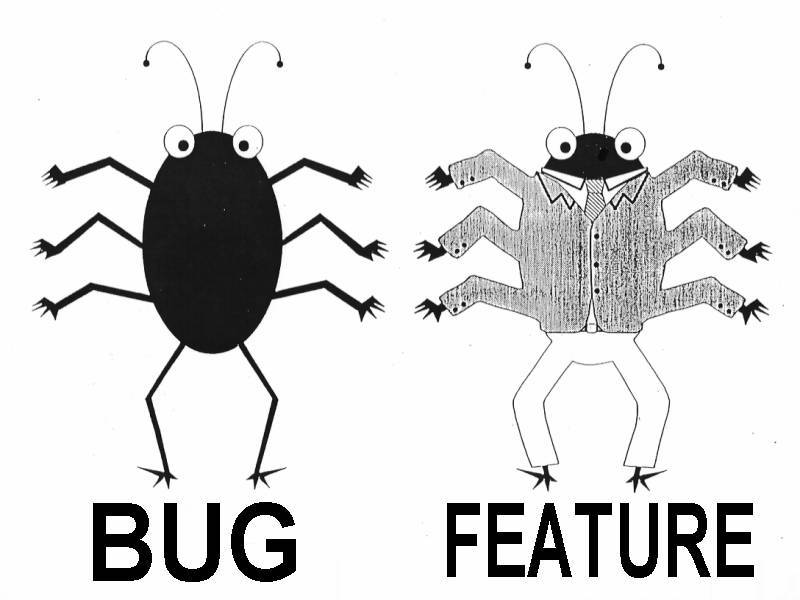
\includegraphics[width=0.3\textwidth]{pics/bugvsfeature.jpg}
    \end{figure}
    \begin{itemize}
      \item Programming is a complex activity
      \item Mistakes happen all the time
      \item A mistake made in programming is called a bug
      \item The process of finding and resolving bugs is called debugging
    \end{itemize}
  \end{block}

  \begin{block}{Errors}
    \begin{itemize}
      \item Syntax error
            \begin{itemize}
              \item Incorrect syntax of a statement: \lstinline!print(Hello World)! instead of \lstinline!print("Hello World")!
            \end{itemize}
      \item Runtime error

            \begin{itemize}
              \item Error that occurs during the execution of a program
              \item e.g. division by 0
            \end{itemize}
      \item Semantic errors
            \begin{itemize}
              \item Program does not deliver correct results
              \item No error messages (code is syntactically correct)
              \item Fixing semantic errors can be extremely complicated (good software design is important)
            \end{itemize}
    \end{itemize}
  \end{block}
  \framebreak
  \begin{block}{Techniques}
    \begin{itemize}
      \item Reading code
      \item Print variables with \lstinline!print()! to examine values (a poor man's debugger)
      \item Go through the program step by step -> \textbf{Debugger}!
    \end{itemize}
  \end{block}



\end{frame}
% subsection naming_conventions_&_debugging (end)

\subsection{Conditionals: if/else/elif} % (fold)
\label{sub:conditionals}

\begin{frame}[c,fragile, allowframebreaks]\frametitle{Conditionals}
  \begin{itemize}
    \item Boolean algebra is a part of mathematics
    \item Often used in programming
    \item A boolean expression is either true or false
  \end{itemize}

  \begin{lstlisting}
5 == 5 # --> True
5 == 6 # --> False
6 > 4 # --> True
5 >= 8 # --> False
\end{lstlisting}

  \framebreak
  {
    \footnotesize

    \begin{examples}

      \begin{block}{\color{mLightBrown}if}

        \begin{itemize}
          \item The expression if defines a condition
          \item If the condition is true, subsequent statements will be executed
          \item If the condition is false, subsequent statements will not be executed
          \item There has to be at least one statement after the condition
        \end{itemize}

      \end{block}
    \end{examples}

    \begin{lstlisting}
x = 10
if x > 0:
  print(f'{x} is positive')
if True:
  # This statement will always be executed
  print('Yes')
if False:
  # This statement will never be executed
  print('No')
\end{lstlisting}
  }
  \framebreak

  \begin{block}{\color{mLightBrown}else}
    \begin{itemize}
      \item Expression else is executed if the if condition is false
      \item Can only be used in combination with an if expression
    \end{itemize}
  \end{block}

  \begin{lstlisting}
if x == 0:
  print('x is zero')
else:
  print('x is not zero')
\end{lstlisting}

  \framebreak

  \begin{examples}
    \begin{block}{\color{mLightBrown}\%-operator (remainder after division)}
      {}
    \end{block}
  \end{examples}
  \begin{lstlisting}
def print_parity(x):
  if x % 2 == 0:
    print('The number is even')
  else:
    print('The number is odd')

print_parity(2)
print_parity(3)
\end{lstlisting}

  \framebreak

  \begin{block}{Chained conditionals}
    \begin{itemize}
      \item \lb{elif} is used to combine multiple conditions
      \item The \lb{else} expression is executed when neither \lb{if} nor any of the \lb{elif}s is true.
      \item Any number of \lb{elif} expressions can be used but only one \lb{if} and one \lb{else}
    \end{itemize}
  \end{block}


  \framebreak

  \begin{examples}
    \begin{lstlisting}
if x < y:
  print(f'{x} is less than {y}')
elif x > y:
  print(f'{x} is greater than {y}')
else:
  print(f'{x} and {y} are equal')
\end{lstlisting}
    \begin{lstlisting}
# Python 3
answer = input('Do you like Python?')
# Python 2.7
# answer = raw_input('Do you like Python?')
if answer == 'yes':
  print('That is great!')
else:
  print('That is disappointing!')
\end{lstlisting}
  \end{examples}
\end{frame}

{
\setbeamercolor{background canvas}{bg=mLightBlue}
\setbeamercolor{frametitle}{fg=white,bg=mLightBlue}
\setbeamercolor{normal text}{fg=white}
\usebeamercolor[fg]{normal text}
\bfseries
\begin{frame}[c]\frametitle{Exercise 1}
  Solve exercise 1
\end{frame}
}

\begin{frame}[c, fragile, allowframebreaks]\frametitle{Conditionals}
  \begin{block}{Nested conditionals}
    \begin{itemize}
      \item Conditionals can be nested
    \end{itemize}
    \begin{lstlisting}
if x > 0:
  if x < 10:
    print('x is a positive single digit')
\end{lstlisting}
  \end{block}
  \begin{block}{\color{mLightBrown}and}
    \begin{itemize}
      \item Deep nesting can be difficult to read
      \item Use \lb{and} to combine conditionals
    \end{itemize}
  \end{block}
  \begin{lstlisting}
if x > 0:
  if x < 10:
    print('x is a positive single digit')
# is the same as
if x > 0 and x < 10:
  print('x is a positive single digit')
\end{lstlisting}


  \bblock{\lb{or}}{

    \begin{itemize}
      \item  At least one statement must be true for the condition to be true
    \end{itemize}
  }

  \begin{lstlisting}
if x > 0 or x < 0:
  print("x is not zero")
\end{lstlisting}

  \bblock{\lb{not}}{
    \begin{itemize}
      \item Negation, inverts the boolean.
      \item \lb{not} True -> becomes False
      \item \lb{not} False -> becomes True
    \end{itemize}
  }

  \begin{lstlisting}
if not (y == 0):
  print(x/y)
else:
  print("Cannot divide by zero")
\end{lstlisting}

  \begin{table}
    \begin{tabular}{p{1cm}*{3}{p{2cm}}}
      \textbf{X} & \textbf{Y} & \textbf{X and Y} & \textbf{X or Y} \\
      \toprule
      False      & False      & False            & False           \\
      False      & True       & False            & True            \\
      True       & False      & False            & True            \\
      True       & True       & True             & True
    \end{tabular}

  \end{table}


\end{frame}
% subsection conditionals (end)
{
\setbeamercolor{background canvas}{bg=mLightBlue}
\setbeamercolor{frametitle}{fg=white,bg=mLightBlue}
\setbeamercolor{normal text}{fg=white}
\usebeamercolor[fg]{normal text}
\bfseries
\begin{frame}[c, fragile]\frametitle{Exercise 2}

  Solve exercise 2
\end{frame}

\begin{frame}[c, fragile]\frametitle{Exercise 3}
  Solve exercise 3
\end{frame}

}
% subsection functions_with_return_values (end)

\subsection{Lists: []} % (fold)
\label{sub:lists}

\begin{frame}[c, fragile, allowframebreaks]\frametitle{Lists}

  \begin{itemize}
    \item Lists are a data type
    \item Lists are used in most programming languages (arrays)
    \item Lists are a set of values
  \end{itemize}

  \begin{lstlisting}
list_a = [1, 2, 4]
list_b = ['Monty', 'Python']
\end{lstlisting}

  \framebreak

  \bblock{Creating lists}{
    \begin{itemize}
      \item The easiest way to create a list is using []
    \end{itemize}
  }

  \begin{lstlisting}
numbers = [10, 12, 14, 19]
words = ['spam', 'bungee', 'swallow']
\end{lstlisting}

  \begin{itemize}
    \item Data types can be mixed
  \end{itemize}

  \begin{lstlisting}
my_list = ['music', 2000, 3.5, True]
\end{lstlisting}

  \framebreak

  \bblock{Creating lists}{
    \begin{itemize}
      \item Since numbers are often stored in a list, there is a special method for doing so
      \item With only one argument, range returns a number series starting at 0
    \end{itemize}
  }

  \begin{lstlisting}
list(range(4))
# returns [0, 1, 2, 3]
\end{lstlisting}

  \begin{itemize}
    \item When using two arguments it is possible to define the start and end of the range $\left[\text{start}, \text{end}\right)$ (end is not included in the list)
  \end{itemize}

  \begin{lstlisting}
list(range(1,5))
# returns [1, 2, 3, 4]
\end{lstlisting}

  \framebreak

  \bblock{Creating lists}{
    \begin{itemize}
      \item The step size can be defined with a third argument
    \end{itemize}
  }

  \begin{lstlisting}
list(range(1, 10, 2))
# return [1, 3, 5, 7, 9]
\end{lstlisting}

  \begin{itemize}
    \item An empty list can also be created
  \end{itemize}

  \begin{lstlisting}
empty_list = []
\end{lstlisting}
  \begin{itemize}
    \item This is often done when the values to be inserted in the list are not yet known.
  \end{itemize}

  \framebreak

  \bblock{Creating lists}{
    \begin{itemize}
      \item Accessing elements can be done with the [] operator
    \end{itemize}
  }

  \begin{lstlisting}
names = ['Anna', 'Tom', 'Ralph', 'Peter']
print(names[1])
# prints Tom
\end{lstlisting}

  \begin{alertblock}{Important}
    Array indices start at 0!
  \end{alertblock}

  \begin{table}
    \begin{tabular}{c|c|c|c}
      0    & 1   & 2     & 3     \\
      \midrule
      Anna & Tom & Ralph & Peter
    \end{tabular}
  \end{table}

  \framebreak

  \bblock{Accessing lists}{
    \begin{itemize}
      \item A negative index is used to access the list from the end
    \end{itemize}
  }

  \begin{lstlisting}
names = ['Anna', 'Tom', 'Ralph', 'Peter']
print(names[-1])
# prints Peter
\end{lstlisting}

  \framebreak

  \bblock{Length}{
    \begin{itemize}
      \item The number of elementsi n a list can be obtained using the \texttt{len()} function
    \end{itemize}
  }

  \begin{lstlisting}
names = ['Anna', 'Tom', 'Ralph', 'Peter']
print(len(names))
# prints 4
\end{lstlisting}

  \bblock{Out of range}{
    \begin{itemize}
      \item If there is no item in the list at the desired index, Python will print an error
            message
    \end{itemize}
  }

  \begin{lstlisting}
names = ['Anna', 'Tom', 'Ralph', 'Peter']
n_names = len(names)
print(names[n_names])
# IndexError: list index out of range
\end{lstlisting}

  \framebreak

  \bblock{Changing elements in a list}{
    \begin{itemize}
      \item An element can be changed using [INDEX]
    \end{itemize}
  }

  \begin{lstlisting}
names = ['Anna', 'Tom', 'Ralph', 'Peter']
names[0] = 'Alice'
# ['Alice', 'Tom', 'Ralph', 'Peter']
\end{lstlisting}

  \framebreak

  \bblock{Adding elements}
  {
    \begin{itemize}
      \item The \texttt{append()} method can be used t o add an element at the end of the list
    \end{itemize}
  }

  \begin{lstlisting}
numbers = list(range(5))
# [0, 1, 2, 3, 4]
numbers.append(5)
# [0, 1, 2, 3, 4, 5]
\end{lstlisting}

  \framebreak

  \bblock{Concatenate lists}{
    \begin{itemize}
      \item The + operator can be used to join lists
    \end{itemize}
  }

  \begin{lstlisting}
a = [1, 2, 3]
b = [4, 5, 6]
c = a + b
# [1, 2, 3, 4, 5, 6]
\end{lstlisting}

  \framebreak

  \bblock{Slices}{
    \begin{itemize}
      \item Lists can be cut into slices
      \item The operator [n:m] returns a list of the elements that start at index n and stop before m
    \end{itemize}
  }

  \begin{lstlisting}
my_list = ['a', 'b', 'c', 'd', 'e', 'f']
my_list[1:3]
# ['b', 'c']
\end{lstlisting}

  \framebreak

  \bblock{Slices}{
    \begin{itemize}
      \item If the first index is empty, the slice starts at the beginning
    \end{itemize}
  }

  \begin{lstlisting}
my_list = ['a', 'b', 'c', 'd', 'e', 'f']
my_list[:4]
# ['a', 'b', 'c', 'd']
\end{lstlisting}

  \begin{itemize}
    \item If the second index is empty, the slice will include elements until the end of the list
  \end{itemize}

  \begin{lstlisting}
my_list = ['a', 'b', 'c', 'd', 'e', 'f']
my_list[3:]
# ['d', 'e', 'f']
\end{lstlisting}

  \framebreak

  \bblock{Deleting elements}{
    \begin{itemize}
      \item The \texttt{del()} method deletes items from the list
    \end{itemize}
  }

  \begin{lstlisting}
list_a = ['one', 'two', 'three']
del(list_a[1])
# ['one', 'three']
list_b = ['a', 'b', 'c', 'd', 'e', 'f']
del(list_b[1:5])
# ['a', 'f']
\end{lstlisting}

\end{frame}
\subsection{Immutables: Tuples () and Strings}
\begin{frame}[c, fragile, allowframebreaks]\frametitle{Tuples}

  \bblock{Tuples is an immutable sequence data type}{
    \begin{itemize}
      \item It is not possible to assign to the individual items of a tuple, however it is possible to create tuples which contain mutable objects, such as lists.
      \item Tuples are declared using () instead of []
    \end{itemize}
  }

  \begin{lstlisting}
tuple = ('a', 'b', 'c', 'd', 'e')
\end{lstlisting}

  \begin{itemize}
    \item Tuples containing only one element (singleton) must have a comma at the end of the definition
  \end{itemize}
  \begin{lstlisting}
tuple = ('a', )
\end{lstlisting}

\end{frame}

\begin{frame}[c, fragile, allowframebreaks]{Strings}

  \bblock{Strings are immutable}{
    \begin{itemize}
      \item Unlike lists, strings cannot be changed
      \item Operations on strings always return a modified copy of the string
      \item The original string remains unchanged
    \end{itemize}
  }

  \begin{lstlisting}
greeting = 'Hello, world!'
greeting[0] = 'J'
# TypeError: 'str' object does not support item assignment
\end{lstlisting}



\end{frame}


% subsection lists (end)

\subsection{Iteration: for/while} % (fold)
\label{sub:iteration}

\begin{frame}[c, fragile, allowframebreaks]\frametitle{Iterations}

  \begin{itemize}
    \item Iterations are used to repeat statements
    \item There are two expressions for iterations
          \begin{itemize}
            \item \lb{while}
            \item \lb{for}
          \end{itemize}
  \end{itemize}

  \bblock{\lb{while}}{
    \begin{itemize}
      \item As long as the condition of the while loop is True, the body of the loop gets executed
    \end{itemize}
  }

  \begin{example}
    \begin{lstlisting}
def countdown(n):
  while n > 0:
    print(n)
    n = n - 1
  print('Lift off!')

countdown(10)
\end{lstlisting}
  \end{example}


  \bblock{\lb{while}}{
    \begin{itemize}
      \item If the condition is False at the beginning, the body of the loop is never executed
      \item If the variable that is used to check the condition of the while loop does not change, the loop will never terminate -> infinite loop
      \item Whether a while loop terminates can be hard to determine
    \end{itemize}
  }

  \begin{lstlisting}
def sequence(n):
  while n != 1:
    print(n)
    if n % 2 == 0:
      n = n / 2
    else:
      n = n * 3 + 1
\end{lstlisting}

  \framebreak

  \bblock{\lb{while}}{
    \begin{itemize}
      \item A \lb{while} loop can be used to iterate through a list
    \end{itemize}
  }

  \begin{lstlisting}
names = ['Tom', 'Anna', 'Christopher']
index = 0
while index < len(names):
  name = names[index]
  print(name)
  index = index + 1
\end{lstlisting}
\end{frame}

{
\setbeamercolor{background canvas}{bg=mLightBlue}
\setbeamercolor{frametitle}{fg=white,bg=mLightBlue}
\setbeamercolor{normal text}{fg=white}
\usebeamercolor[fg]{normal text}
\bfseries
\begin{frame}[c, fragile]\frametitle{Exercise 4}

  Solve exercise 4
\end{frame}

}

{
\setbeamercolor{background canvas}{bg=mLightBlue}
\setbeamercolor{frametitle}{fg=white,bg=mLightBlue}
\setbeamercolor{normal text}{fg=white}
\usebeamercolor[fg]{normal text}
\bfseries
\begin{frame}[c, fragile]\frametitle{Exercise 5}

  Solve exercise 5
\end{frame}

}

\begin{frame}[c, fragile]\frametitle{Iterations}

  \bblock{\lb{for}}{
    \begin{itemize}
      \item Since it is often necessary to operate through lists and other data types, there is a special expression for this
    \end{itemize}
  }

  \begin{lstlisting}
for element in element_list:
  print(element)
  \end{lstlisting}


\end{frame}

{
\setbeamercolor{background canvas}{bg=mLightBlue}
\setbeamercolor{frametitle}{fg=white,bg=mLightBlue}
\setbeamercolor{normal text}{fg=white}
\usebeamercolor[fg]{normal text}
\bfseries
\begin{frame}[c, fragile]\frametitle{Exercise 6}
  Solve exercise 6
\end{frame}
}

% subsection iteration (end)

\subsection{Dictionaries: \{\}} % (fold)
\label{sub:dictionaries}

\begin{frame}[c, allowframebreaks, fragile]\frametitle{Dictionaries}

  \bblock{Key-Value pair}{
    \begin{itemize}
      \item Dictionaries are very similar to lists but have a key and value for each entry
      \item The entries of a dictionary are not sorted
    \end{itemize}
  }

  \framebreak

  \bblock{Creating dictionaries}{
    \begin{itemize}
      \item Dictionaries are created using \{\}
    \end{itemize}
  }

  \begin{lstlisting}
eng2de = {}
eng2de['one'] = 'eins'
eng2de['two'] = 'zwei'
\end{lstlisting}

  \begin{itemize}
    \item Values can be added directly
  \end{itemize}

  \begin{lstlisting}
inventory = {
'apples': 430,
'bananas': 312,
}
\end{lstlisting}

  \framebreak

  \bblock{Accessing entries}{
    \begin{itemize}
      \item Values can be accessed directly using dictionary['key']
    \end{itemize}
  }

  \begin{lstlisting}
inventory = {
'apples': 430,
'bananas': 312,
}
print(inventory['apples'])
# 430
\end{lstlisting}

  \framebreak

  \bblock{Assigning and modifying values}{
    \begin{itemize}
      \item The key is assigned a value
      \item If the key already exists the existing value is overwritten
    \end{itemize}
  }

  \begin{lstlisting}
inventory = {
'apples': 430,
'bananas': 312,
}
inventory['oranges'] = 530
inventory['bananas'] = 250
print(inventory['bananas'])
# 250
\end{lstlisting}

  \framebreak

  \bblock{Deleting entries}{
    \begin{itemize}
      \item Key-Value pairs can be delted using the \texttt{del()} function
    \end{itemize}
  }

  \begin{lstlisting}
inventory = {
'apples': 430,
'bananas': 312,
}
del(inventory['bananas'])
\end{lstlisting}

  \framebreak

  \bblock{Number of entries}{
    \begin{itemize}
      \item The \texttt{len()} function returns the number of entries
    \end{itemize}
  }

  \begin{lstlisting}
inventory = {
  'apples': 430,
  'bananas': 312,
}
len(inventory)
# 2
\end{lstlisting}

  \framebreak

  \bblock{Checking if an entry exists}{
    \begin{itemize}
      \item The \lb{in} keyword can be used to check if a key exists in a dictionary
    \end{itemize}
  }

  \begin{lstlisting}
inventory = {
  'apples': 430,
  'bananas': 312,
}
if 'apples' in inventory:
  inventory['apples'] += 100
else:
  inventory['apples'] = 100
\end{lstlisting}

  \framebreak

  \bblock{Iterating over entries}{
    \begin{itemize}
      \item The \texttt{items()} function combined with the \lb{for} statement can be used to iterate through every key-value pair
    \end{itemize}
  }

  \begin{lstlisting}
for (my_key, my_value) in my_dict.items():
  print(my_key + ' : ' + my_value)
\end{lstlisting}

\end{frame}

{
\setbeamercolor{background canvas}{bg=mLightBlue}
\setbeamercolor{frametitle}{fg=white,bg=mLightBlue}
\setbeamercolor{normal text}{fg=white}
\usebeamercolor[fg]{normal text}
\bfseries
\begin{frame}[c]\frametitle{Exercise 7}
  Solve exercise 7
\end{frame}

\begin{frame}[c]\frametitle{Exercise 8}
  Solve exercise 8
\end{frame}

\begin{frame}[c, fragile]\frametitle{Exercise 9}
  Solve exercise 9
\end{frame}

}

% subsection dictionaries (end)
% section fundamental_concepts (end)

\section{Persistence} % (fold)
\label{sec:persistence}

\begin{frame}[c, fragile]\frametitle{Persistence}
  \begin{itemize}
    \item So far no data has been saved in any of our examples
    \item All data was deleted from the memory as soon as our examples quit
    \item There are several ways to permanently store data on the hard disk
          \begin{itemize}
            \item Database
            \item Simple text files
          \end{itemize}
  \end{itemize}
\end{frame}


\begin{frame}[c, fragile, allowframebreaks]\frametitle{Files}

  \bblock{Common procedure}{
    \begin{itemize}
      \item Open file
      \item Do something with the file
      \item Close the file - depending on syntax done automatically.
    \end{itemize}
  }

  \begin{lstlisting}
with open('my_file.txt', 'mode') as file:
  # do some stuff
\end{lstlisting}

  \framebreak

  \bblock{Different modes}{
    \begin{itemize}
      \item The mode defines how the content of the file should be treated
      \item Modes
            \item'r': read only
            \item'w': write only
            \item'r+': read and write
            \item'a': append
    \end{itemize}
  }

  \begin{lstlisting}
# open a file in read/write mode
with open('my_file.txt', 'r') as file:
  # do some stuff
\end{lstlisting}

  \framebreak

  \bblock{Write}{
    \begin{itemize}
      \item The write() function is used to write something into a file
      \item \lb{'\textbackslash n'} is used to insert a line break
    \end{itemize}
  }

  \begin{lstlisting}
with open('my_file.txt', 'a') as file:
  file.write('First line of the write operation')
  file.write('This is a line with a new-line character at the end\n')
  file.write('This is another line, on a new-line below the previous one.\n')
\end{lstlisting}

  \framebreak

  \bblock{Read}{
    \begin{itemize}
      \item A \lb{for} loop can be used to read a file line by line
      \item \texttt{line.strip()} removes the trailing \lb{'\textbackslash n'}
    \end{itemize}
  }

  \begin{lstlisting}
with open('my_file.txt', 'r') as file:
  for line in file:
    line = line.strip()
    print(line)
\end{lstlisting}
\end{frame}

\begin{frame}[c, fragile, allowframebreaks]\frametitle{JSON}

  \bblock{Dictionaries/list in JSON}{
    \begin{itemize}
      \item file.write() only accepts strings as arguments
      \item If complex structures such as dictionaries or lists should be stored in a file, it’s necessary the convert these structures into strings first
      \item An example of a standard used for this purpose is JSON (Javascript Object Notation)
    \end{itemize}
  }

  \begin{lstlisting}
import json
my_dict = {'one': 'eins', 'two': 'zwei'}
my_dict_as_string = json.dumps(my_dict)
print(my_dict_as_string)
\end{lstlisting}

  \framebreak

  \bblock{Convert JSON to dictionaries/lists}{
    \begin{itemize}
      \item Example of a string in JSON that is converted into a dictionary
    \end{itemize}
  }

  \begin{lstlisting}
import json
my_dict_as_string = '{"two": "zwei", "one": "eins"}'
my_dict = json.loads(my_dict_as_string)
print(my_dict)
\end{lstlisting}

\end{frame}

{
\setbeamercolor{background canvas}{bg=mLightBlue}
\setbeamercolor{frametitle}{fg=white,bg=mLightBlue}
\setbeamercolor{normal text}{fg=white}
\usebeamercolor[fg]{normal text}
\bfseries
\begin{frame}[c, fragile]\frametitle{Exercise 10}
  Solve exercise 10
\end{frame}
}
% section persistence (end)

\begin{frame}[c]\frametitle{Additional Resources}
  \begin{itemize}
    \item How to Think Like a Computer Scientist from Allen Downey, Jeffrey Elkner, and Chris Meyers
    \item Learning with Python: Interactive Edition 2.0
          \begin{itemize}
            \item \url{http://interactivepython.org/courselib/static/thinkcspy/index.html}
          \end{itemize}

    \item Official Python Documentation
          \begin{itemize}
            \item \url{http://www.python.org/doc/}
          \end{itemize}

    \item Project Euler: Mathematical problems that can be solved
          programmatically
          \begin{itemize}
            \item \url{http://projecteuler.net/}
          \end{itemize}

    \item Platforms to prepare for coding interviews
          \begin{itemize}
            \item \url{https://leetcode.com}
            \item \url{https://www.interviewbit.com/}
          \end{itemize}

  \end{itemize}

\end{frame}

\end{document}
